% vim: set textwidth=78 autoindent:

\section{Uso dei Plugin Core QGIS}\label{sec:core_plugins}\index{plugin!core}

% when the revision of a section has been finalized, 
% comment out the following line:
%\updatedisclaimer

QGIS \CURRENT contiene 22 plugin di base che possono essere caricati tramite
il QGIS Plugin Manager (vedi la tabella \ref{tab:core_plugins}).

% minipage is needed to appear the footnote under the table
% SH
\begin{minipage}{\textwidth}
\begin{table}[H]
\centering
\caption{QGIS Core Plugins}\label{tab:core_plugins}\medskip
\small
 \begin{tabular}{|l|l|p{4in}|}
\hline \textbf{Icon} & \textbf{Plugin} & \textbf{Description}\\
\hline

\includegraphics[width=0.6cm]{delimited_text}
 & Aggiungi layer testo delimitato \index{plugin!testo delimitato} & Carica e mostra file di testo delimitato contenenti coordinate x,y\\
\hline

\includegraphics[width=0.6cm]{coordinate_capture}
 & Cattura Coordinate \index{plugin!cattura coordinate}& Cattura le coordinate del mouse
usando SRS diverso\\
\hline 
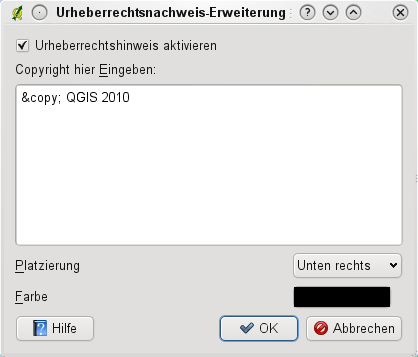
\includegraphics[width=0.6cm]{copyright_label}
 & Etichetta di copyright \index{plugin!etichetta diritti d'autore}& Disegna una etichetta diritti d'autore con informazioni\\
\hline 

\includegraphics[width=0.6cm]{diagram_overlay}
 & Diagramma sovrapposto \index{plugins!diagramma}& Disegna un grafico (a torta o barre) o simboli proporzionali sopra un layer vettoriale\\
\hline

\includegraphics[width=0.6cm]{dxf2shp_converter}
 & DXF2Shape Convertitore \index{plugin!convertitore DXF2Shape}& Converte da formato DXF a SHP\\
\hline
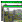
\includegraphics[width=0.6cm]{evis_icon}
 & eVis & Strumento di visualizzazione di eventi \\
\hline

\includegraphics[width=0.6cm, height=0.6cm]{ftoolslogo}
 & fTools \index{plugins!ftools}& Insieme di strumenti per l'analisi, la geometria, l'elaborazione e la ricerca\\
\hline

\includegraphics[width=0.6cm]{gps_importer}
 & Strumenti GPS \index{plugin!GPS}& Strumenti per caricare e importare dati GPS\\
\hline

\includegraphics[width=0.6cm]{grass}
 & GRASS \index{plugin!strumenti GRASS} & Attiva i potenti strumenti di GRASS\\
\hline
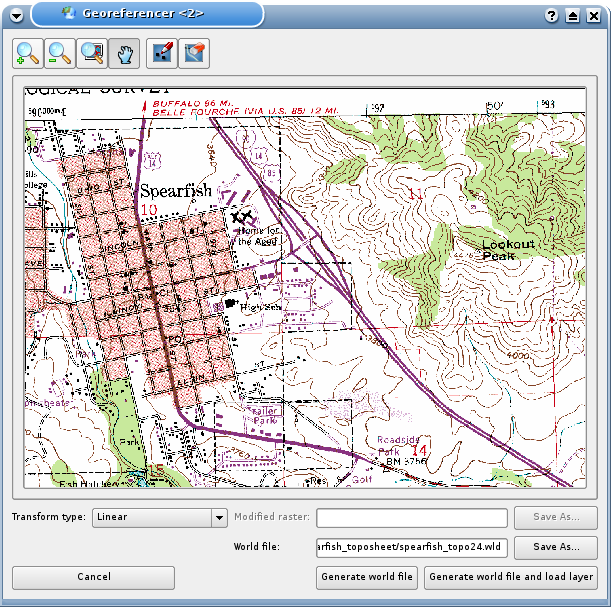
\includegraphics[width=0.6cm]{georeferencer}
 & Georeferenziatore \index{plugin!georeferenziatore} & Aggiunge proiezioni ai file raster\\
\hline

\includegraphics[width=0.6cm]{interpolation}
& Plugin di Interpolazione \index{plugin!interpolazione}& Interpolazione basata sui vertici di un layer vettoriale\\
\hline

\includegraphics[width=0.6cm]{raster_terrain}
& Analisi geomorfologia Raster \index{plugins!Analisi morfologia raster}& Calcola pendenza, esposizione,
indice di asperità e curvatura totale dei DEM\\
\hline

\includegraphics[width=0.6cm]{mapserver_export}
& Plugin MapServer Export \index{plugin!esportazione verso MapServer}& Esporta un progetto QGIS
in un file mappa MapServer \\
\hline
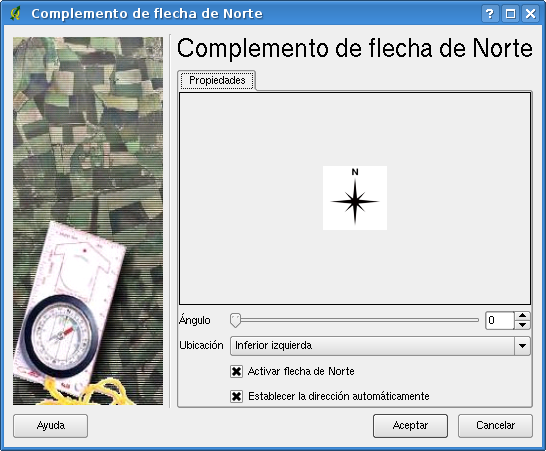
\includegraphics[width=0.6cm]{north_arrow}
& Freccia nord \index{plugin!freccia nord}& Mostra una freccia che indica il nord sovrapposto alla mappa\\
\hline

\includegraphics[width=0.6cm]{ogr_converter}
 & Convertitore di layer OGR \index{plugin!convertitore OGR} & Traduce i layer vettoriali tra formati supportati OGR\\
\hline
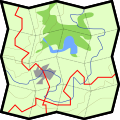
\includegraphics[width=0.6cm]{osm_icon}
 & OpenStreetMap & Visualizza e modifica dati OpenStreetMap \\
\hline

\includegraphics[width=0.6cm]{oracle_raster}
 & Oracle Georaster \index{plugins!georaster}& Accedi a Oracle Spatial GeoRasters\\
\hline

\includegraphics[width=0.6cm]{plugin_installer}
 & Installatore di Plugin \index{plugin!installatore plugin Python} & Scarica e installa i plugin QGIS python\\
\hline

\includegraphics[width=0.6cm]{spiticon}
 & SPIT \index{plugin!SPIT}& Strumento di importazione di file shape in PostgreSQL/PostGIS \\
\hline

\includegraphics[width=0.6cm]{quick_print}
 & Stampa veloce \index{plugin!stampa veloce}& Stampa rapidamente una mappa con sforzo minimo \\
\hline
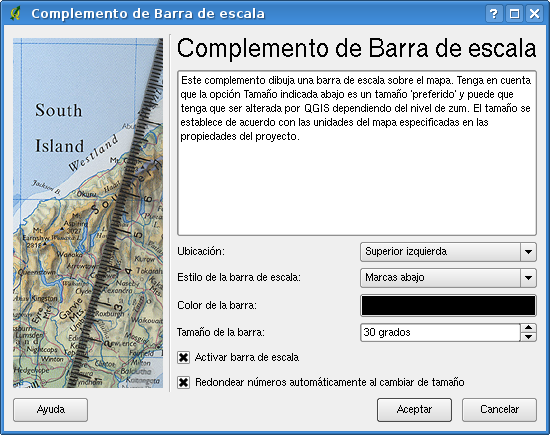
\includegraphics[width=0.6cm]{scale_bar}
 & Barra di Scala \index{plugin!barra di scala}& Disegna una barra di scala\\
\hline

\includegraphics[width=0.6cm]{mIconAddWfsLayer}
 & WFS & Carica e mostra un layer WFS\\
\hline
\end{tabular}
\end{table}
\end{minipage}

\normalsize

